\documentclass[12pt]{article}
\usepackage[utf8]{inputenc}
\usepackage[T1]{fontenc}
\usepackage{amsmath}
\usepackage{amsfonts}
\usepackage{amssymb}
\usepackage[version=4]{mhchem}
\usepackage{stmaryrd}
\usepackage{graphicx}
\usepackage{physics}

\usepackage{listings} % Required for insertion of code
\usepackage{xcolor} % Required for custom colors

% Define custom colors
\definecolor{codegreen}{rgb}{0,0.6,0}
\definecolor{codegray}{rgb}{0.5,0.5,0.5}
\definecolor{codepurple}{rgb}{0.58,0,0.82}
\definecolor{backcolour}{rgb}{0.95,0.95,0.92}

% Setup the style for code listings
\lstdefinestyle{mystyle}{
    backgroundcolor=\color{backcolour},   
    commentstyle=\color{codegreen},
    keywordstyle=\color{magenta},
    numberstyle=\tiny\color{codegray},
    stringstyle=\color{codepurple},
    basicstyle=\ttfamily\footnotesize,
    breakatwhitespace=false,         
    breaklines=true,                 
    captionpos=b,                    
    keepspaces=true,                 
    numbers=left,                    
    numbersep=5pt,                  
    showspaces=false,                
    showstringspaces=false,
    showtabs=false,                  
    tabsize=2
}

% Activate the style
\lstset{style=mystyle}

\graphicspath{{./images/}}


\title{Assignment 3: Quantum statistical mechanics and thermalization }


\author{Instructor: Lesik Motrunich\\
TA: Liam O'Brien}
\date{}


\begin{document}
\maketitle
Ph 121C: Computational Physics Lab, Spring 2024

California Institute of Technology

Due: 4 pm Tuesday, May 14, 2024

\section*{1 Introduction to quantum thermalization}
In this assignment we broaden our focus, previously restricted to ground and low-energy states, to include the entire spectrum as well as the time evolution of quantum states under a manybody Hamiltonian. While time evolution as governed by the Schrödinger equation is perhaps not too difficult for a single particle (i.e., quantum mechanics), in an interacting system of many constituents the situation is evidently much more complicated. Composite classical systems are described on macroscopic scales by statistical mechanics, but we do not have a formal connection between this theory and the microscopic physics. For this reason many questions remain open: one example is the problem of deriving thermodynamic irreversibility - the general tendency to approach equilibrium-from microscopic equations which are symmetric in time. However, it seems essential for the validity of statistical mechanics that a system explores its entire microscopic phase space (subject to constraints like energy conservation) given enough time, a property called ergodicity. The natural mechanism for ergodicity is chaotic dynamics, in which similar initial microscopic configurations diverge exponentially quickly in time under the nonlinear equations of motion governing the constituents.

The analogous quantum situation is the time evolution of an isolated pure state of a manybody system, referred to as a quench. As the equation of motion for a closed quantum system is linear, chaos of the type encountered classically is prohibited. In addition, the unitarity of the time evolution operator $\exp (-i t H)$ requires the dynamics to be strictly reversible, as the initial state of a quantum system can be reconstructed from the state at later times by the application of the backwards-time operator with $t \mapsto-t$. It was paradoxical, then, when in the early 1990s both Srednicki and Deutsch proposed that an isolated quantum system under time evolution does indeed generically approach a type of equilibrium thermal state, independent of both the properties of the initial state and the fine details of the Hamiltonian, similar to the case in classical statistical mechanics. Moreover, this was predicted to occur in isolated states in the absence of coupling to a thermal bath or any kind of reservoir.

Subsequent numerical simulations as well as analytic work and experimental evidence support the claim, now known as the eigenstate thermalization hypothesis (ETH), in a variety of quantum systems. As we will see, there are multiple ways to understand the phenomenon of quantum thermalization, including by examining those cases where ETH is violated. In the following we will explore both ETH and non-ETH dynamics using exact diagonalization of spin systems similar to the quantum Ising model with which you are already familiar.

\section*{2 Eigenstate thermalization hypothesis}
\subsection*{2.1 Quantum chaos}
As described above, the linearity of Schrödinger's equation prohibits the exponential divergence of trajectories in phase space which is the signature of chaotic dynamics. In fact, we cannot really make a direct comparison because the uncertainty principle prohibits localizing quantum states in phase space; however, we note that time evolution actually preserves overlaps:


\begin{equation*}
\langle\phi(t) \mid \psi(t)\rangle=\left\langle\phi(0)\left|U^{\dagger}(t) U(t)\right| \psi(0)\right\rangle=\langle\phi(0) \mid \psi(0)\rangle \tag{1}
\end{equation*}


The modern understanding of quantum chaos is due to work from the 1960s and 1970s when Wigner and others were studying the spectra of large atomic nuclei. These energy eigenvalues, while experimentally measurable, had too complicated a structure to describe with an analytic form; instead, Wigner's insight was that if one focuses on a small energy window the Hamiltonian looks like a matrix with random entries when represented in a generic basis. Thus, the eigenvalues of quantum Hamiltonians at finite energy density should be described by the statistical properties of random matrices, subject to some physical symmetry constraints. This topic is known as random matrix theory (RMT), and is quite successful in describing energy eigenvalues, particularly via "level statistics." RMT also predicts that the eigenvectors of such Hamiltonians look nearly stochastic, and moreover turn out to be very sensitive to small perturbations; thus a slightly perturbed Hamiltonian written in the unperturbed eigenbasis already looks again like a random matrix. Because the eigenvectors of the Hamiltonian are the stationary states of the system, this is understood as the quantum counterpart to classical exponentially diverging trajectories.

\subsection*{2.2 Dynamical ETH}
The canonical picture of classical thermalization involves a small (finite) system in contact with an infinitely large reservoir. Over time, the smaller system will come to equilibrium with the reservoir through the transfer of energy by various microscopic processes, which are not themselves important. Initially, the smaller system may have certain distinct characteristics, such as a particular profile for its energy density or magnetization, but these are lost as the system reaches equilibrium and takes on the average properties of the reservoir. That is, after a sufficiently long time, the only relevant quantity is in fact the temperature $\tau$ of the reservoir, and the system explores its microstates according to the Boltzmann distribution, which associates a probability $p(\varepsilon) \propto e^{-\beta \varepsilon}$ with a microstate of energy $\varepsilon$ (here, $\beta=1 / \tau$ ). In particular, the reverse process is exceedingly unlikely: a system in equilibrium is not expected to reconstruct its initial conditions before a time which is doubly exponential in the system size. This is known as the Poincaré recurrence time.

One formulation of ETH is the claim that the thermalization behavior described above applies also to small subsystems of an isolated quantum system in the thermodynamic limit undergoing time evolution. We will make this statement more precise by considering the expectation values of local observables, supported on a few sites, in the time-evolving quantum state. Let $|\psi(0)\rangle=\sum_{n} c_{n}|n\rangle$\\
be some initial state along with its decomposition in the eigenbasis of $H,\{|n\rangle\}_{n=1, \ldots, 2^{N}}$. In this basis, the time-evolved state is


\begin{equation*}
|\psi(t)\rangle=\sum_{n} c_{n} e^{-i \varepsilon_{n} t}|n\rangle \tag{2}
\end{equation*}


where $\varepsilon_{n}$ is the energy eigenvalue corresponding to $|n\rangle$. Now suppose that we measure some local observable $O$ in the state as a function of time. Its expectation value is given by


\begin{align*}
O(t) \equiv\langle\psi(t)|O| \psi(t)\rangle & =\sum_{m, n} c_{m}^{*} c_{n} e^{-i\left(\varepsilon_{n}-\varepsilon_{m}\right) t}\langle m|O| n\rangle  \tag{3}\\
& =\sum_{n}\left|c_{n}\right|^{2} O_{n n}+\sum_{m, n \neq m} c_{m}^{*} c_{n} e^{-i\left(\varepsilon_{n}-\varepsilon_{m}\right) t} O_{m n} \tag{4}
\end{align*}


Taking a long-time average of the observable, and absent degeneracies in the spectrum, the offdiagonal terms in (4) will be eliminated by dephasing; thus, the time average will approach the time-independent value given by the first sum, which is based only on the initial conditions. In this sense, equilibration is actually a generic feature of quantum quenches.

The statement of ETH is much stronger, however: not only do local observables $O$ equilibrate in time, but they approach a specific thermal value. Recall that we may appeal to RMT when focused on a narrow energy window, say of width $\delta$; this corresponds to an initial state $|\psi(0)\rangle$ with only small energy fluctuations. Then the predicted thermal value of the operator is in fact its average in the eigenstates within the energy window:


\begin{equation*}
O_{\mathrm{MC}}=\frac{1}{N_{\varepsilon \pm \delta}} \sum_{\left\{n:\left|\varepsilon_{n}-\varepsilon\right|<\delta\right\}} O_{n n} \tag{5}
\end{equation*}


where $N_{\varepsilon \pm \delta}$ is the number of eigenstates $|n\rangle$ with energy $\left|\varepsilon_{n}-\varepsilon\right|<\delta$. This is the average used to measure quantities in the microcanonical ensemble in statistical mechanics. This picture can be extended to make a broader claim about the spectrum in the case that the only conserved (local) quantity in the system is the energy. Then the prediction of ETH is the measurement corresponding to a "Gibbs state:"


\begin{equation*}
O_{\beta}=\frac{1}{Z_{\beta}} \operatorname{tr}\left[e^{-\beta H} O\right] \tag{6}
\end{equation*}


where the partition function $Z_{\beta}=\operatorname{tr}\left[e^{-\beta H}\right]$. This is the average in the canonical ensemble at temperature $\tau=1 / \beta$. To be more precise, strong ETH is the claim that for any local observable and any initial state, in the thermodynamic limit the late-time value approaches the form (6). Another formulation, weak ETH, also asserts the above but only for typical-or "almost all"local observables and initial states.

By probing local observables time-evolving under an interacting Hamiltonian from initial states with low entanglement, we emulate the classical picture of thermalization between a small system (the support of the operator) and a reservoir (the remainder of the sites). However, in doing so we actually provide the resolution of the paradox between late-time equilibration and the reversibility of unitary dynamics. It turns out that the information about the initial state is not lost in the equilibrium state, but instead is "smeared out" from its initial configuration and becomes encoded nonlocally in the time-evolved state. Operators acting on extensively many sites, then, will not appear thermal even after local observables have equilibrated, and reversing the dynamics restores the initial state by again localizing the information specific to the initial condition. The apparent directionality of the quench is based on the choice of an initial state having low entanglement, which contains very little information in extensive operators and as we saw in the previous assignment is atypical in the full Hilbert space.

\subsection*{2.3 Eigenstate ETH}
The arguments of the previous section lead to a paradox: if the long-time behavior of an observable $O$ is given by the diagonal terms of (4), which depend on the initial state, how can it approach the universal form given by (5)? The resolution is that dynamical ETH is equivalent to thermalization of the eigenstates - hence the name - which is to say that expectation values of operators in an eigenstate at energy $\varepsilon_{n}$ are essentially determined by the thermal value (6) at the corresponding $\beta\left(\varepsilon_{n}\right)$. The precise statement for the matrix elements of local operators in the energy eigenbasis is


\begin{equation*}
O_{m n}=O_{\beta}\left(\varepsilon_{n}\right) \delta_{m n}+e^{-S(\bar{\varepsilon}) / 2} f_{O}\left(\varepsilon_{m}, \varepsilon_{n}\right) R_{m n} \tag{7}
\end{equation*}


where $\bar{\varepsilon}$ is the average of $\varepsilon_{m}$ and $\varepsilon_{n}, S$ the thermodynamic entropy, and $f_{O}(\cdot, \cdot)$ is some smooth function modulating a random variable $R_{m n}$. It is essential that $O_{\beta}\left(\varepsilon_{n}\right)$ is a smooth function, and for (5) to hold, measurements in nearby eigenstates should look nearly the same: $O_{n+1, n+1}-O_{n, n}$ is exponentially small in system size in the middle of the spectrum, where energies $\varepsilon_{n}$ and $\varepsilon_{n+1}$ are also exponentially close.

However, the arguments for thermalization do not apply near the edges of the spectrum: these distinguished energy regions generally behave quite differently from the rest of the eigenstates, which has been a recurring theme in the previous assignments. In particular, the density of states is lower at the band edges, and so heuristically it is more difficult for eigenstates to "hybridize" with one another as the Hamiltonian is perturbed. Recall the values of the ground state fidelity you found in Assignment 1 for the gapped phases of the Ising model; these should have been nearly 1 and thus represent a clear violation of the prediction of RMT applied to the ground state.

\section*{3 Failure to thermalize}
One very interesting question is, what are the limits of the picture described above? That is, do all systems exhibit thermalization, or are there some necessary assumptions that can be violated? The avoidance of thermalization has important real-world implications, for example for quantum information devices that need to be shielded from decoherence. It turns out that in principle certain Hamiltonians can indeed avoid thermalization. These fall into two classes which superficially are quite different, but turn out to have a similar underlying property which prevent initial states from reaching equilibrium, namely that the evolution is strongly constrained by conservation laws.

\subsection*{3.1 Integrable quantum systems}
An integrable system is one respecting an extensive number of conserved quantities, or local integrals of motion. These conservation laws restrict the dynamics to such an extent that, once identified, they allow exact solution of the model. For example, the one-dimensional quantum Ising model in a transverse field is integrable. This is seen by mapping to spinless fermions through the JordanWigner transformation, which results in a free theory of particles hopping on a lattice. The model is solved independently for each of the fermionic momentum states; then, generating multi-particle states simply corresponds to setting the occupation of each of the single-particle orbitals.

In such a system thermalization is avoided due to the non-interaction of the constituents. More generally, two-body interacting models can also be integrable if the interaction terms satisfy a particular condition known as the Yang-Baxter equation. The addition of a longitudinal field $\sum_{j} \sigma_{j}^{x}$ to the Ising model breaks its integrability, introducing an interaction term (between the fermions) of the type that eliminates the conservation of single-particle states.

\subsection*{3.2 Many-body localization}
Recently, a great deal of study has been devoted to a newer mechanism of avoided thermalization, which is known as many-body localization (MBL). MBL is a phenomenon in which fixed randomness (so-called "quenched disorder," not to be confused with the previous usage of quench) in some of the terms in the Hamiltonian causes all eigenstates of an interacting system to become localized, with a transition from delocalized to localized eigenstates occurring at some finite strength of the disorder.

Since Anderson, it has been known that disorder in a non-interacting system will result in localization of the single-particle states, which may either occur for arbitrarily weak disorder or else above some transition value. However, it is conventionally expected that allowing interactions leads to resonances which delocalize the many-body states, presumably following ETH as in the quantum integrable case when interactions are introduced. Instead, numerical evidence indicates that above a localization transition, strong disorder localizes all eigenstates. This transition to MBL is qualitatively different from the quantum phase transitions we studied previously, as it occurs throughout the entire spectrum.

In order to understand MBL, one can refer to "l-bits," which are emergent local integrals of motion (for weak disorder they can be thought of as dressed spins with exponential tails); because extensively many of these appear, they provide a basis for approximate diagonalization of the system. In this way MBL systems avoid thermalization by a mechanism related to integrable systems, with conservation laws arising from (and particular to) a disorder realization.

\section*{4 Assignment: quantum statistical mechanics and thermalization}
\subsection*{4.1 Dynamical ETH}
Set up dense exact diagonalization for the quantum Ising model in a field with both transverse and longitudinal components:


\begin{equation*}
H=-J \sum_{j=1}^{L} \sigma_{j}^{z} \sigma_{j+1}^{z}-h^{x} \sum_{j=1}^{L} \sigma_{j}^{x}-h^{z} \sum_{j=1}^{L} \sigma_{j}^{z} \tag{8}
\end{equation*}


For simplicity, set $J=1$. You should use periodic b.c. throughout the assignment to minimize finite-size effects. We are not so concerned with the ground state of the system or its low-energy states; what is important is that any $h^{z} \neq 0$ breaks the integrability of the transverse-field Ising model, thus we expect ETH behavior. We will use the particular values $\left(h^{x}, h^{z}\right)=(-1.05,0.5)$, which specify a sufficiently generic point in the parameter space.

\subsection*{4.1.1 Time evolution of an initial state}
We wish to choose an initial state with average energy from somewhere near the middle of the energy spectrum. As thermalization is a general feature, this choice should not be too important, but it can affect the early-time behavior, or the time required to reach the thermal state. For simplicity, use a translation-invariant product state:


\begin{equation*}
|\psi(t=0)\rangle=|\xi\rangle_{1} \otimes|\xi\rangle_{2} \otimes \cdots \otimes|\xi\rangle_{L}, \quad|\xi\rangle=\frac{1}{2}(|\uparrow\rangle-\sqrt{3}|\downarrow\rangle) \tag{9}
\end{equation*}


First, diagonalize $H$ for the parameter values specified in the previous section using various system sizes $L=8,10,12,14$. Use the eigenstates of $H$ you computed to expand the initial state\\
$|\psi(t=0)\rangle$ in the energy eigenbasis. That is, calculate the coefficients $c_{n}$ of $|\psi(t=0)\rangle=\sum_{n=1}^{2^{L}} c_{n}|n\rangle$, where $n$ indexes the eigenstates $|n\rangle$ of $H$, with energy eigenvalues $\varepsilon_{n}$. At this point we could compute the time-evolved state according to (2); however, it turns out we do not even need to explicitly perform this calculation. We can instead directly evolve the expectation value itself in time via the expression (3). Use this method, and plot the time dependence of the observables $\left\langle\sigma_{1}^{\mu}(t)\right\rangle$, $\mu=x, y, z$, for each system size $L$ (the choice of site is arbitrary, due to translation invariance). Time-evolve for long enough to observe a qualitative change in the observables' behavior, using a short enough step size $\delta t$ to give a smooth curve. Based on your data, what behavior do you expect as $L \rightarrow \infty$ ? At late times you may observe a seeming return to a state like the initial one. This is not a Poincaré recurrence - which occurs only after doubly-exponentially long times - but rather a finite-size effect arising from "wavefronts" reaching the boundaries of the system and bouncing back and forth, or circling the entire system in the periodic case.
\newpage
I was only able to glow several system sizes of 4, 6, 8, and 10. A dampening effect can be seen as we move towards longer times for the larger system sizes, followed by a recurrence in the maturation. The presence of this dampening effect was more prominent for larger system sizes, so I expect that the behavior in the infinite system limit would be to approach the thermal equilibrium value for the given observable at large times.
\begin{figure}
    \centering
    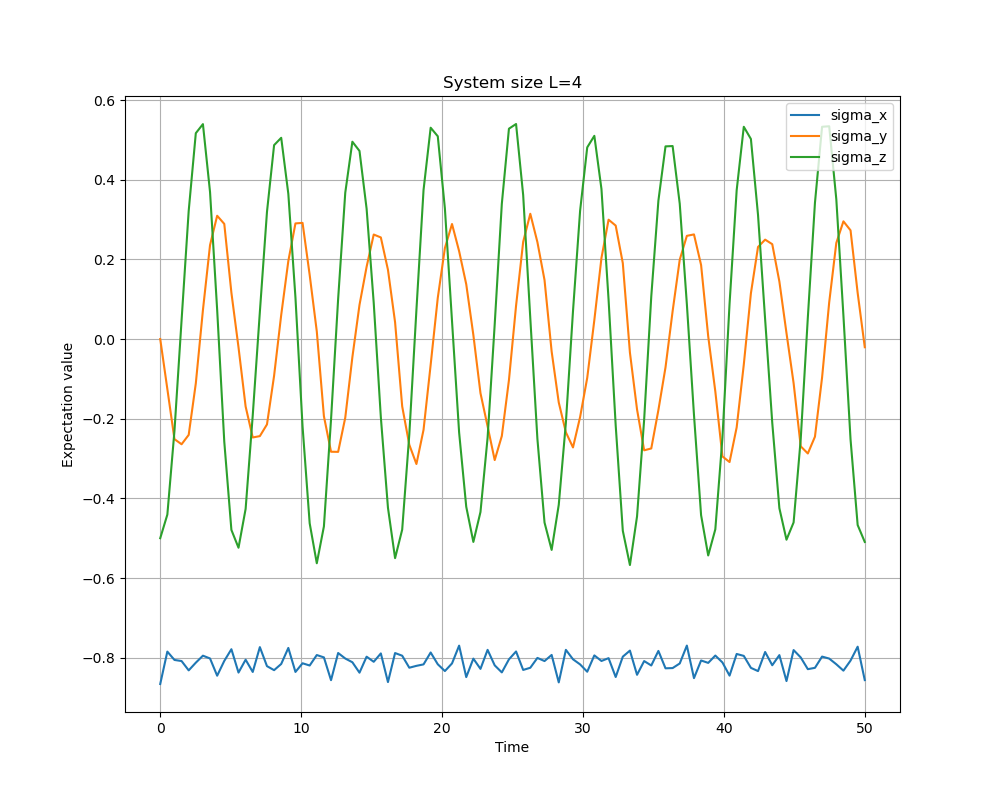
\includegraphics[width=\textwidth]{Expectation_values_L_4.png}
    \caption{Expectation values for system size L=4}
\end{figure}
\begin{figure}
    \centering
    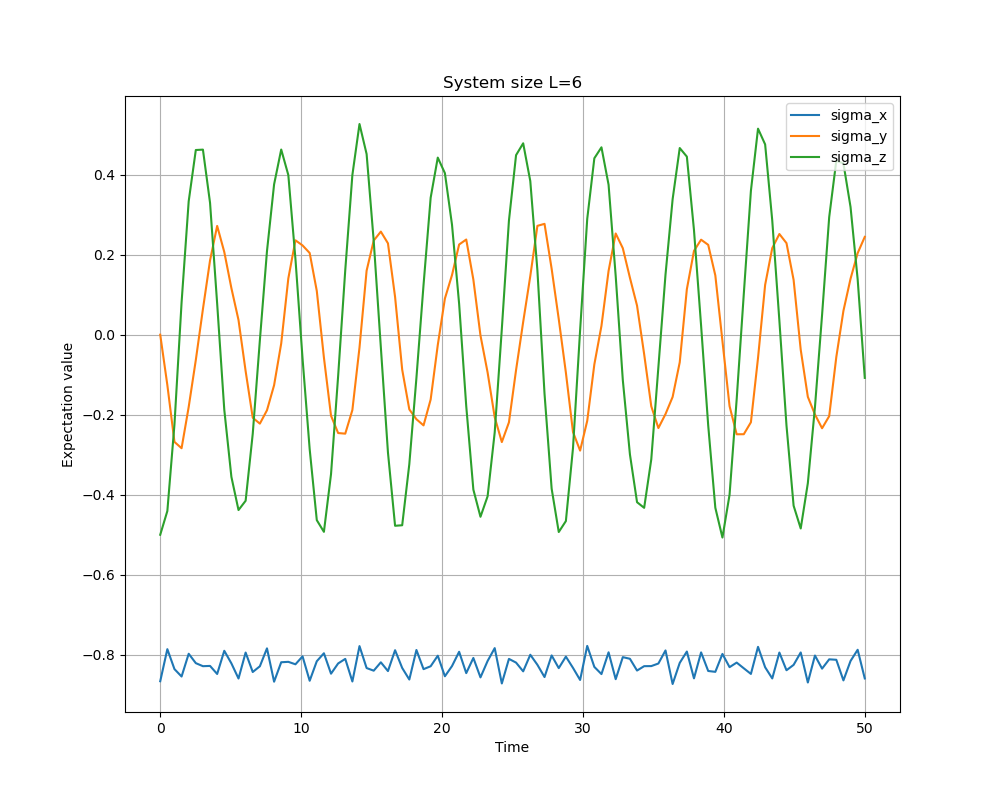
\includegraphics[width=\textwidth]{Expectation_values_L_6.png}
    \caption{Expectation values for system size L=6}
\end{figure}
\begin{figure}
    \centering
    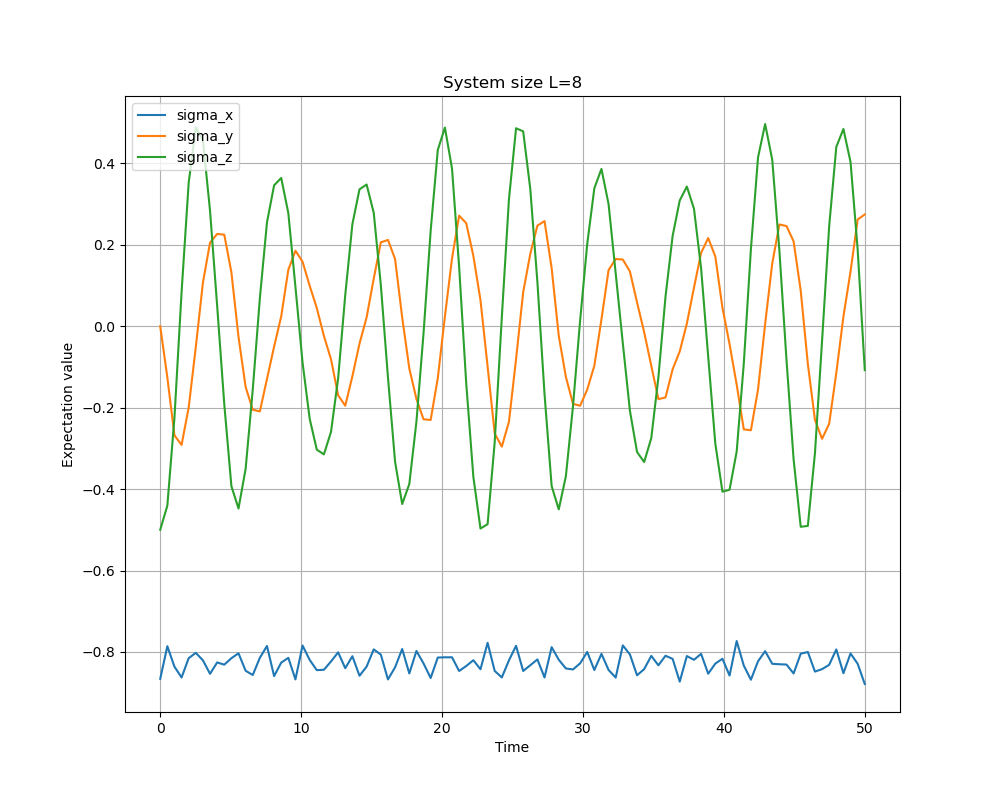
\includegraphics[width=\textwidth]{Expectation_values_L_8.png}
    \caption{Expectation values for system size L=8}
\end{figure}
\begin{figure}
    \centering
    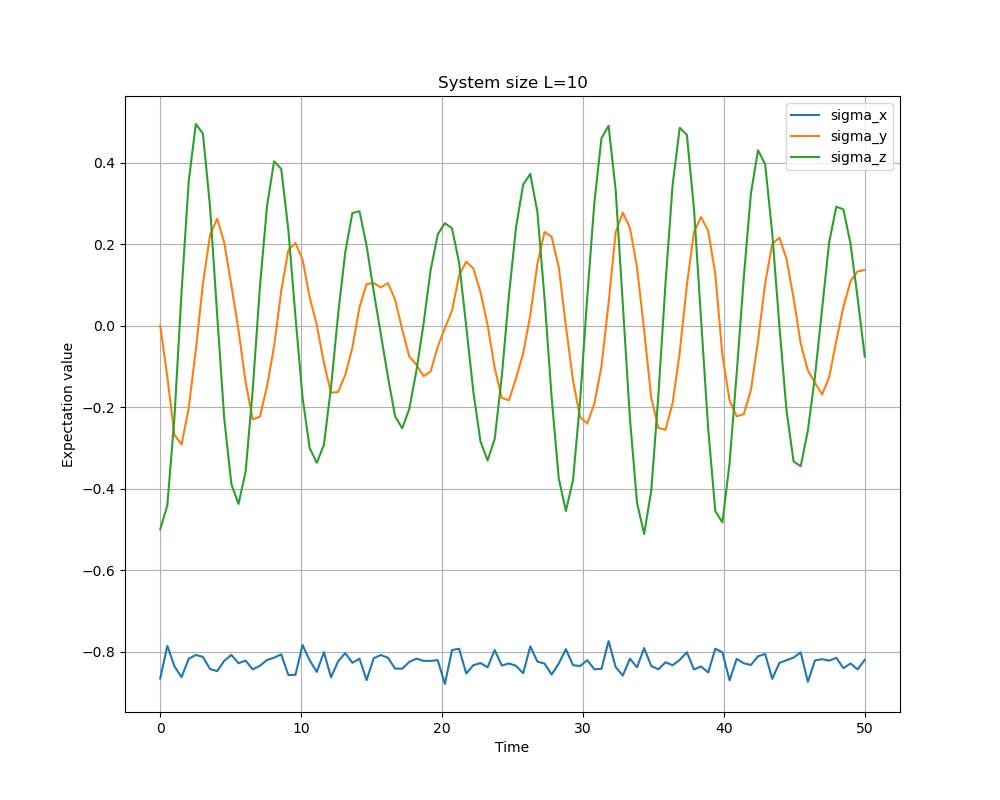
\includegraphics[width=\textwidth]{Expectation_values_L_10.png}
    \caption{Expectation values for system size L=10}
\end{figure}
% Inline Python code in the document
\begin{lstlisting}[language=Python]
import numpy as np
import matplotlib.pyplot as plt
from hw1.src.hw1 import tensor_product, periodic_dense_hamiltonian_explicit

# now construct something like O(t) \equiv\langle\psi(t)|O| \psi(t)\rangle & =\sum_{m, n} c_{m}^{*} c_{n} e^{-i\left(\varepsilon_{n}-\varepsilon_{m}\right) t}\langle m|O| n\rangle  \tag{3}\\
def compute_observable_expectation_vectorized(t, observable, overlap_coefficients, eigenvalues, eigenvectors):
    # Precompute matrix elements
    observable_eigenvectors = np.dot(observable, eigenvectors)
    matrix_elements = np.dot(eigenvectors.conj().T, observable_eigenvectors)
    
    # Compute phase factors
    energy_diffs = eigenvalues[:, None] - eigenvalues[None, :]
    phase_factors = np.exp(-1j * energy_diffs * t)
    
    # Compute weights from overlap coefficients
    weight_matrix = overlap_coefficients[:, None] * overlap_coefficients.conj()[None, :]
    
    # Combine all to compute expectation
    return np.sum(weight_matrix * phase_factors * matrix_elements)


# System size and parameters
L_values = [4, 6, 8, 10]
h_x = -1.05
h_z = 0.5
t_values = np.linspace(0, 50, 100)  # More time points for a smoother curve

# Define the observables for the first site
sigma_x = np.array([[0, 1], [1, 0]])
sigma_y = np.array([[0, -1j], [1j, 0]])
sigma_z = np.array([[1, 0], [0, -1]])
identity = np.identity(2)

# Dictionary to hold plots for legends
observables_labels = ['sigma_x', 'sigma_y', 'sigma_z']

for L in L_values:
    # Extend observables to the full system size
    full_observables = {
        'sigma_x': tensor_product([sigma_x] + [identity] * (L - 1)),
        'sigma_y': tensor_product([sigma_y] + [identity] * (L - 1)),
        'sigma_z': tensor_product([sigma_z] + [identity] * (L - 1))
    }
    
    # Initial state: tensor product of single_site across all sites
    single_site = np.array([1, -np.sqrt(3)]) / 2
    initial_state = single_site.copy()  # Start with a copy of single_site

    for _ in range(1, L):
        initial_state = np.kron(initial_state, single_site)  # Properly extending to the full system size

    
    # Prepare to plot
    plt.figure(figsize=(10, 8))
    plt.title(f"System size L={L}")
    plt.xlabel("Time")
    plt.ylabel("Expectation value")

    # Generate the Hamiltonian
    H = periodic_dense_hamiltonian_explicit(L, h_x, h_z)

    # Diagonalize the Hamiltonian
    eigenvalues, eigenvectors = np.linalg.eigh(H)

    # calculate the overlap coefficients
    overlap_coefficients = np.dot(eigenvectors.conj().T, initial_state)

    for label, observable in full_observables.items():
        expectations = []
        for t in t_values:
            print(L, label)
            expectation = compute_observable_expectation_vectorized(t, observable, overlap_coefficients, eigenvalues, eigenvectors)
            expectations.append(np.real(expectation))  # Using real part; adjust if needed

        plt.plot(t_values, expectations, label=label)

    plt.legend()
    plt.grid(True)
    plt.savefig(f"Expectation_values_L_{L}.png")
\end{lstlisting}

\subsection*{4.1.2 Thermal values of observables}
It is evident from (2) that the energy of the state $E=\langle\psi(0)|H| \psi(0)\rangle$ does not change with time, and in fact energy is the only conserved quantity in the Hamiltonian (8). Thus we should use $E$ to determine the asymptotic temperature of the equilibrium thermal state. To do so, plot the thermal state energy


\begin{equation*}
E_{\beta}=\frac{1}{Z_{\beta}} \operatorname{tr}\left[H e^{-\beta H}\right]=\frac{1}{Z_{\beta}} \sum_{n} e^{-\beta \varepsilon_{n}}\langle n|H| n\rangle=\frac{1}{Z_{\beta}} \sum_{n} e^{-\beta \varepsilon_{n}} \varepsilon_{n} \tag{10}
\end{equation*}


As a function of $\beta$ for each $L$, you can then match these values with the energy $E$ of the initial state in order to determine the corresponding inverse temperature $\beta$ of the equilibrium state.
\newpage
I computed the thermal energy as a function of beta and then I computed the initial state energy that is conserved in order to determine the corresponding inverse temperature beta of the equilibrium state.

\begin{figure}
    \centering
    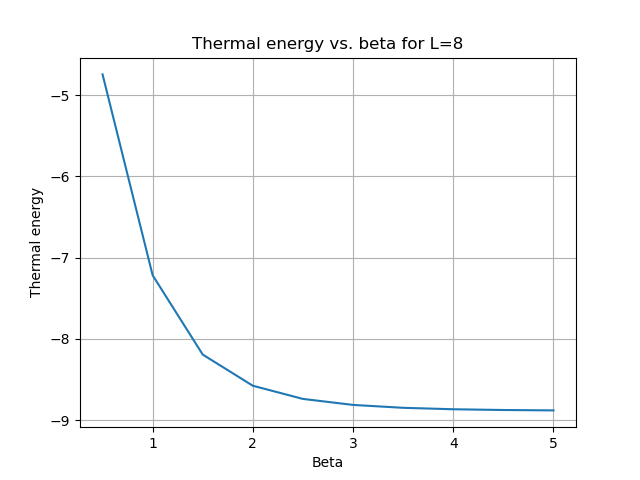
\includegraphics[width=\textwidth]{p4_1_2_L8.png}
    \caption{Thermal energy as a function of beta for system size L=8. The energy of the initial state is marked with a horizontal line.}
\end{figure}
% Inline Python code in the document
\begin{lstlisting}[language=Python]
import numpy as np
import matplotlib.pyplot as plt
from hw1.src.hw1 import tensor_product, periodic_dense_hamiltonian_explicit
from p4_1 import compute_observable_expectation_vectorized


def compute_thermal_energy(beta, eigenvalues):
    """
    Compute the thermal energy of a system characterized by size L at inverse temperature beta.
    
    Parameters:
    - beta: Inverse temperature.
    - L: System size.
    
    Returns:
    - thermal_energy: The thermal energy of the system.
    """
    # Compute the partition function
    Z = sum(np.exp(-beta * eigenvalues))
    
    # Initialize thermal energy
    thermal_energy = 0
    
    # Iterate over all energy levels
    for i in range(len(eigenvalues)):
        thermal_energy += eigenvalues[i] * np.exp(-beta * eigenvalues[i])
    # Divide by the partition function
    thermal_energy /= Z
    return thermal_energy


def compute_thermal_observable(beta, eigenvalues, eigenvectors, observable):
    """
    Compute the thermal expectation value of an observable.
    
    Parameters:
    - beta: Inverse temperature.
    - eigenvalues: Eigenvalues from the Hamiltonian diagonalization.
    - eigenvectors: Eigenvectors from the Hamiltonian diagonalization.
    - observable: The observable matrix.
    
    Returns:
    - thermal_observable: The thermal expectation value of the observable.
    """
    # Compute the Boltzmann factors for each eigenstate
    boltzmann_factors = np.exp(-beta * eigenvalues)
    
    # Compute the observable in the eigenbasis
    observable_in_basis = eigenvectors.conj().T @ observable @ eigenvectors
    
    # Compute the weighted trace of the observable
    weighted_trace = np.sum(boltzmann_factors * np.diag(observable_in_basis))
    
    # Compute the partition function Z
    Z = np.sum(boltzmann_factors)
    
    # Calculate the thermal observable
    thermal_observable = weighted_trace / Z
    
    return thermal_observable

def make_product_state(single_site, L):
    """
    Generate the product state for a system of size L.
    
    Parameters:
    - single_site: The state of a single site.
    - L: The size of the system.
    
    Returns:
    - product_state: The product state of the system.
    """
    product_state = single_site.copy()
    for _ in range(1, L):
        product_state = np.kron(product_state, single_site)
    return product_state

# Set system parameters
L_values = [4, 6, 8, 10]
h_x = -1.05
h_z = 0.5
beta_values = np.linspace(0.5, 3, 20)

# Define simple matrices
sigma_x = np.array([[0, 1], [1, 0]])
sigma_y = np.array([[0, -1j], [1j, 0]])
sigma_z = np.array([[1, 0], [0, -1]])
identity = np.identity(2)
observables_labels = [f"sigma_{label}" for label in ['x', 'y', 'z']]

for l in L_values:
    # Generate the Hamiltonian
    H = periodic_dense_hamiltonian_explicit(l, h_x, h_z)
    # Diagonalize the Hamiltonian
    eigenvalues, eigenvectors = np.linalg.eigh(H)

    # Compute thermal energies
    thermal_energies = {}
    for beta in beta_values:
        thermal_energies[beta] = compute_thermal_energy(beta, eigenvalues)

    plt.figure()
    plt.title(f"Thermal Energy vs. $\\beta$ for L={l}")
    plt.xlabel(r"$\beta$")
    plt.ylabel("Thermal Energy")
    plt.plot(list(thermal_energies.keys()), list(thermal_energies.values()))
    plt.grid()

    # Generate the initial state
    initial_state = make_product_state(np.array([1, -np.sqrt(3)] / 2), l)
    
    # Calculate the overlap coefficients
    overlap_coefficients = np.dot(eigenvectors.conj().T, initial_state)

    # Compute the initial energy of the initial state
    initial_energy = compute_observable_expectation_vectorized(0, H, overlap_coefficients, eigenvalues, eigenvectors)

    # Plot the horizontal dashed red line at the initial energy
    plt.axhline(y=initial_energy, color='r', linestyle='--', label="Initial Energy")

    # Find and annotate the intersection point
    intersection_found = False
    for beta, energy in thermal_energies.items():
        if abs(energy - initial_energy) < 1e-1:
            plt.annotate(rf"$\beta = {beta:.2f}$", (beta, energy), textcoords="offset points", xytext=(0, 10), ha='center', color='red')
            intersection_found = True
            beta_intersection = beta
            break

    if not intersection_found:
        plt.annotate("No intersection found", (beta_values[-1], initial_energy), textcoords="offset points", xytext=(-40, -10), ha='center', color='red')

    # Add legend and save the plot
    plt.legend()
    plt.savefig(f"p4_1_2_L{l}.png")
\end{lstlisting}
Now measure the same observables $\left\langle\sigma_{1}^{\mu}\right\rangle_{\beta}, \mu=x, y, z$, in the equilibrium state using (6) and compare these to your time-dependent values by marking these values as horizontal lines on your time trace of $\left\langle\sigma_{1}^{\mu}(t)\right\rangle$. Comment on the approach to equilibrium and the dependence on system size. You will notice that one of the $\left\langle\sigma_{1}^{\mu}\right\rangle_{\beta}$ disappears identically. Which one is this, and why?
\newpage
Again, as time goes on, there is an approach to the equilibrium value for the observables, which is the same phenomenon as the damping that I mentioned earlier. I notice that the $\left\langle\sigma_{1}^{y}\right\rangle_{\beta}$ observable disappears identically. This can be justified as follows:
\begin{equation}
\bra{\Psi } \sigma_{1}^{y} \ket{\Psi} = i \bra{\Psi } 
\begin{pmatrix}
0 & -1 \\
1 & 0
\end{pmatrix}
\ket{\Psi} = i \mathbb{R}
\end{equation}
so this observable has a purely imaginary expectation value, and so it shows of as a horizontal line with a value of 0 in the plot.
\subsection*{4.1.3 Entanglement entropy growth with time}
The initial state $|\psi(0)\rangle$ has highly excited energy, lying near the middle of the spectrum. However, because it's a product state and therefore very atypical, one may wonder whether under unitary time evolution the property of low entanglement might be preserved in any way. Compute the time-dependent state $|\psi(t)\rangle$ using (2) and measure the half-system entanglement entropy $S_{L / 2}(t)$. Plot the time trace of this quantity, and comment on the behavior at both early and late times. To ensure that we've not accidentally chosen a special excited state, repeat this experiment for some other product state. What are the implications of your measurements with regard to our ability to simulate the time evolution of quantum states using MPS?

\subsection*{4.2 Eigenstate ETH}
\subsection*{4.2.1 Observables in excited states}
In Sec. 4.1 .1 you computed the expectation values $\left\langle\sigma_{1}^{\mu}\right\rangle_{n}, \mu=x, y, z$, in each eigenstate $n$ of the Hamiltonian. ETH predicts that the value of each observable depends only on the energy of the eigenstate, indirectly through the temperature of the Gibbs ensemble. To confirm this we can plot the expectation values of the observables directly as a function of the energy eigenvalue $\varepsilon_{n}$.\\
The situation is different now, because we want to consider the expectation values in the eigenstates of the Hamiltonian, not the time-evolved state.
This looks like:
\begin{equation}
\left\langle\sigma_{1}^{\mu}\right\rangle_{n}=\bra{n}\sigma_{1}^{\mu}\ket{n}
\end{equation}

First however, recall that the initial state $|\psi(0)\rangle$ is translation invariant. Under a translation invariant Hamiltonian on a periodic system, momentum is well-defined; this state occupies the\\
$k=0$ momentum sector. You may have noticed that many of the $c_{n}$ in the expansion of $|\psi(0)\rangle$ in the eigenbasis were exactly 0 ; these correspond to eigenstates in other momentum sectors, which are orthogonal to this state. Hence we want to consider only eigenstates with $k=0$; to identify these we could in principle observe the overlaps $c_{n}$, but this depends on specific details of the initial state and is difficult for larger $L$. A better method is use the translation operator $T$, which shifts the entire system by 1 site: $T\left|\sigma_{1}, \sigma_{2}, \sigma_{3} \ldots, \sigma_{L}\right\rangle=\left|\sigma_{L}, \sigma_{1}, \sigma_{2}, \ldots, \sigma_{L-1}\right\rangle$. The $k=0$ sector can be identified by $\langle n|T| n\rangle=+1$; a matrix element that is any other phase, including -1 , indicates a state from another sector.

Using $T$ to filter the eigenstates, plot the expectation values $\left\langle\sigma_{1}^{\mu}\right\rangle_{n}$ for all $|n\rangle$ in the $k=0$ momentum sector as a function of $\varepsilon_{n} / L$. Plot the data on top of each other for the various system sizes $L$. How does the behavior depend on $\varepsilon_{n} / L$, and how does this change with increasing $L$ ?

[ADDED: A couple of technical remarks on using T: First, you might wonder why you are finding normalized Hamiltonian eigenstates $|n\rangle$ with $|\langle n|T| n\rangle|<1$, which means that they are not eigenstates of the translation operator and seems to be contradiction. These can arise here because states with $k$ and $-k$ are degenerate, and without resolving the momentum explicitly, your black-box diagonalizer will likely find superpositions of these; observing $|\langle n|T| n\rangle|<1$ is thus also a signature that these are not states with zero momentum. Second, to be precise in the ETH analysis, one needs to resolve also the inversion symmetry of the Hamiltonian, e.g., inversion in the middle point of the system, $I\left|\sigma_{1}, \sigma_{2}, \ldots, \sigma_{L-1}, \sigma_{L}\right\rangle=\left|\sigma_{L}, \sigma_{L-1}, \ldots, \sigma_{2}, \sigma_{1}\right\rangle$ (all other inversions can be generated by combining this with translations) and restrict to specific inversion quantum number sector, here $I=+1$ since this is the quantum number of $|\psi(0)\rangle$. Since this is expected to have a smaller effect than resolving the momentum, it is ok not to worry about the inversion symmetry in this assignment, or you can do a more brute-force treatment by filtering the energy eigenstates by their non-zero vs zero overlap with $|\psi(0)\rangle$ (remembering that the computer is unlikely to return exact zero, but a number close to machine precision is likely an exact zero).]

Optional. Also compare these results (for $L=14$ ) with $\left\langle\sigma_{1}^{\mu}\right\rangle(\beta)$, the expectation values in the thermal state at inverse temperature $\beta$, plotted versus $E(\beta) / L=\langle H\rangle(\beta) / L$ as you vary $\beta$. This time when you calculate finite-temperature ensemble averages, use only $k=0$ states for both the numerator and denominator $Z(\beta)$ in (6). This may help to reduce finite-size effects in the calculation. Which values of $\beta$ are associated with which regions of the energy spectrum?

\subsection*{4.2.2 Entropic signature of thermalization}
In addition to the measurements of local observables in eigenstates, compute the half-system entanglement entropy for all $k=0$ sector eigenstates and plot the quantity $S_{L / 2} / L$ as a function of $\varepsilon_{n} / L$ for all system sizes $L$. What dependence on the energy density do you observe, and how does this depend on system size?

Optional. We have been borrowing intuition throughout this assignment from equilibrium statistical mechanics to describe quantum systems. We can test the wisdom of this approach by comparing quantum entanglement entropy with entropy in its original sense: thermodynamic entropy,

which in the canonical ensemble takes the form $S_{\text {th }}(\beta)=-\sum_{n} w_{n}^{(\beta)} \log w_{n}^{(\beta)}$, $w_{n}^{(\beta)}=e^{-\beta \varepsilon_{n}} / Z_{\beta}$. For $L=14$, plot both $S_{L / 2} /(L / 2)$ versus $\varepsilon_{n} / L$ for eigenstates $n$ as well as the thermodynamic entropy $S_{\text {th }}(\beta) / L$ versus $\langle H\rangle(\beta) / L$ by varying $\beta$. Is it appropriate to use the same word "entropy" to describe both quantities?

\subsection*{4.3 Violations of ETH}
\subsection*{4.3.1 Many-body localized model}
We now introduce quenched disorder to the magnetic field terms in the Hamiltonian (8), resulting in an MBL phase. That is, consider


\begin{equation*}
H=-J \sum_{j=1}^{L} \sigma_{j}^{z} \sigma_{j+1}^{z}-\sum_{j=1}^{L} h_{j}^{x} \sigma_{j}^{x}-\sum_{j=1}^{L} h_{j}^{z} \sigma_{j}^{z} \tag{11}
\end{equation*}


Again set $J=1$, but now sample $h_{j}^{x}$ and $h_{j}^{z}$ independently from the uniform distribution over $[-W, W]$. For strong enough $W$ the model is MBL; for a start, you can try $W=3$. Repeat the dynamics experiments you performed above for the ETH system, including the time evolution of observables with reference to the proper thermal state value. Note that the temperature of the "equilibrium" thermal state will be different from the previous case, and depends on your disorder realization.

You should again measure local observables in the eigenstates as well as entanglement entropy, as you did for ETH (however, now there is no translation invariance, so no momentum sectors). You may wish to perform some averaging over disorder realizations for these eigenstate properties, in order to obtain a clearer picture of the behavior. Comment on the measurable difference between ETH and MBL physics.

\subsection*{4.3.2 Quantum many-body scar states}
This topic was first described only very recently and has attracted much interest due to its implications for our understanding of quantum chaos. The concept of a (single-particle) quantum scar state has been known for some time, and is based on the phenomenon of periodic orbits in classical chaotic systems, which can exist in principle but are unstable to small perturbations. By passing to the quantum analog of a classical chaotic system, one finds that certain eigenstates display a "scar," a nonergodic signature similar to the classical case. However, such a pattern was not expected beyond single-particle dynamics; in many-body systems at high energy, a quantum scar state would provide a sharp contrast between the validities of strong and weak ETH.

Therefore, it was surprising when such states were apparently observed in experiments with cold Rydberg atoms. While the Hamiltonian for these systems is tricky due to a complicated structure in the Hilbert space, we can instead study a toy model, the following spin-1/2 Hamiltonian [1):


\begin{equation*}
H=\frac{\Omega}{2} \sum_{j=1}^{L} \sigma_{j}^{x}+\sum_{j=1}^{L} P_{j, j+1} \sigma_{j+2}^{z} \tag{12}
\end{equation*}


where $P_{j, j+1}=\left(1-\boldsymbol{\sigma}_{j} \cdot \boldsymbol{\sigma}_{j+1}\right) / 4$ projects onto the singlet subspace of sites $j$ and $j+1$. Note that the mechanisms of avoided thermalization are absent: (12) is neither disordered nor integrable (the latter can be seen from the Jordan-Wigner transformation). Thus one expects ETH to apply.

In order to fully break the internal spin-rotation symmetry, $H$ contains a three-site term which at first may seem tedious to code. However, recall that $\sigma_{j+2}^{z}$ is diagonal in the standard basis for the many-body Hilbert space, and its effect is to contribute a sign to the matrix elements of the two-body term $P_{j, j+1}$. Thus, you can focus on the nonzero matrix elements of only the two-body operator, and afterward simply add a sign based on the parity of spin $j+2$.

In order to observe the scar states, you should compute the half-system entanglement entropy for the entire spectrum as in Sec. 4.2.2, however now you will observe several states which are\\
evidently far less entangled than the typical eigenstate. For this simple model, the number and exact energies of the scar states are known, indexed by $m=\{-L / 2,-L / 2+1, \ldots, L / 2-1, L / 2\}$ (that is, the $S^{z}$ spin states of an overall spin $s=L / 2$ system), with harmonically spaced energies $E_{m}=\Omega m$. Indicate these energy values on your plot.

Optional. Though the scar states are relatively unentangled, they still may display volume-law scaling with a smaller prefactor. Using several system sizes, try to determine the scaling with $L$ of the scar state entanglement entropy. Do you find evidence for an area law, volume law, or logarithmic scaling?

\subsection*{4.3.3 Optional. Integrable Ising model and GGE}
An integrable model can be obtained by setting $h^{z}=0$ in the translation invariant Hamiltonian (8), recovering the transverse-field quantum Ising model. This model will not equilibrate to a thermal state, but it has been proposed that such a system does reach a state that is a natural generalization, obtained by taking the conservation laws into account. This equilibrium state is known as the generalized Gibbs ensemble (GGE). As this is a somewhat more technical area, we will not go into more detail regarding the GGE, but you may make direct comparisons with the previous cases by again repeating the dynamical and eigenstate experiments of Secs. 4.1 and 4.2 . You may also look into existing numerical results on the GGE to gain intuition about what to expect in this case.

\section*{References}
[1] Choi, Soonwon, Christopher J. Turner, Hannes Pichler, Wen Wei Ho, Alexios A. Michailidis, Zlatko Papić, Maksym Serbyn, Mikhail D. Lukin, and Dmitry A. Abanin. "Emergent SU(2) dynamics and perfect quantum many-body scars." Physical review letters 122, no. 22 (2019): 220603.


\end{document}